
 {\tmstrong{Objective: Identify the equation of a line given a parallel or
perpendicular line.}}\pp

 There is an interesting connection between the slopes of lines that are
parallel, as well as the slopes of lines that are perpendicular (meet at a right
angle). This is shown in the following example.

\begin{example}\label{Lin68}
~\end{example}

  \begin{multicols}{2}
    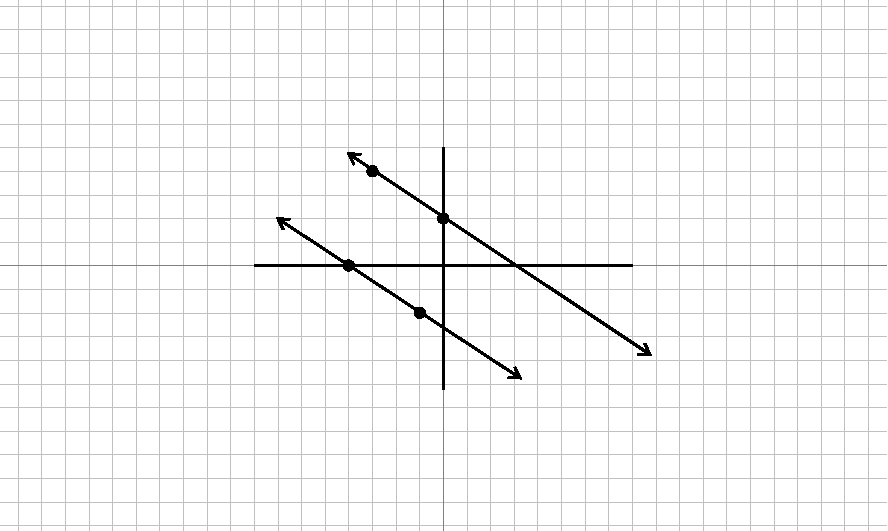
\includegraphics[scale=.9,bb = 115 65 310 190, clip=true]{II_1_5-1.eps}
    
     The above graph has two parallel lines. The slope of the top line is down
    2, run 3, or $- \frac{2}{3}$.\\
		The slope of the bottom line is down 2, run 3 as well, or $- \frac{2}{3}$.
    
    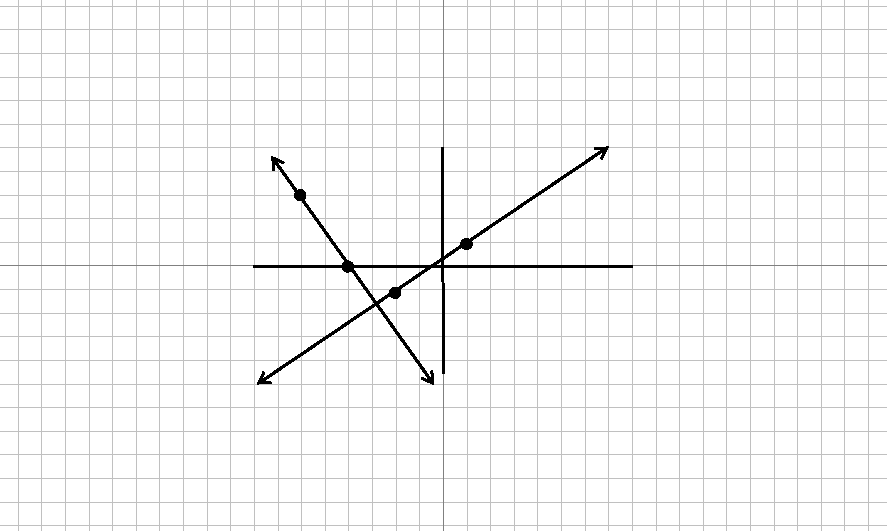
\includegraphics[scale=.9,bb = 115 65 310 190, clip=true]{II_1_5-2.eps}
    
     The above graph has two perpendicular lines. The slope of the flatter line
    is up 2, run 3 or $\frac{2}{3}$.\\
		The slope of the steeper line is down 3, run 2, or $- \frac{3}{2}$.
  \end{multicols}
%\end{example}
~\par

 As the first graph above illustrates, parallel lines have the same slope.\pp
On the other hand, perpendicular lines are said to have \textit{negative reciprocal} slopes.   More precisely, if two lines with slopes $m_1$ and $m_2$ are known to be perpendicular, then $m_2=-~\displaystyle\frac{1}{m_1}$ (and so, $m_1m_2=-1$).\pp
We can use these properties to make conclusions about parallel and perpendicular lines.\pp

{\tmstrong{World View Note:}} Greek Mathematician Euclid lived around 300 BC
and published a book titled, {\tmem{The Elements}}. In it is the famous
parallel postulate which mathematicians have tried for years to drop from the
list of postulates. The attempts have failed, yet all the work done has
developed new types of geometries!\pp

\begin{example}\label{Lin69}~~~Find the slope of a line parallel to $5 y - 2 x = 7$.
  \begin{eqnarray*}
    5 y - 2 x = 7~~~~~ &  & \tmop{To} \tmop{find} \tmop{the} \tmop{slope} \tmop{we}
    \tmop{will} \tmop{put} \tmop{equation} \tmop{in} \tmop{slope} -
    \tmop{intercept} \tmop{form}\\
    \tmmathbf{\underline{+ 2 x ~~ + 2 x}} &  & \tmop{Add} 2 x \tmop{to} \tmop{both}
    \tmop{sides}\\
    5 y = 2 x + 7~~~~~ &  & \tmop{Put} x \tmop{term} \tmop{first}\\
    \tmmathbf{\overline{5} ~~~~ \overline{5} ~~~~~ \overline{5}}~~~~~ &  & \tmop{Divide} \tmop{each}
    \tmop{term} \tmop{by} 5\\
    y = \frac{2}{5} x + \frac{7}{5}~~~~~ &  & \tmop{The} \tmop{slope} \tmop{is}
    \tmop{the} \tmop{coefficient} \tmop{of} x\\
    &  & \\
    m = \frac{2}{5}~~~~~ &  & \tmop{Slope} \tmop{of} \tmop{given} \tmop{line}\\
		& & \tmop{Parallel} \tmop{lines} \tmop{have} \tmop{the} \tmop{same}
    \tmop{slope}\\
    &  & \\
    m = \frac{2}{5}~~~~~ &  & \tmop{Our} \tmop{solution}
  \end{eqnarray*}
\end{example}

\begin{example}\label{Lin70}~~~Find the slope of a line perpendicular to $3 x - 4 y = 2$.
  \begin{eqnarray*}
    3 x - 4 y = 2~~~~ &  & \tmop{To} \tmop{find} \tmop{slope} \tmop{we}
    \tmop{will} \tmop{put} \tmop{equation} \tmop{in} \tmop{slope} -
    \tmop{intercept} \tmop{form}\\
    \tmmathbf{\underline{- 3 x ~~~~~~~~- 3 x}} &  & \tmop{Subtract} 3 x \tmop{from} \tmop{both}
    \tmop{sides}\\
    - 4 y = - 3 x + 2~~~~~ &  & \tmop{Put} x \tmop{term} \tmop{first}\\
    \tmmathbf{\overline{- 4} ~~~ \overline{- 4} ~~ \overline{- 4}}~~~~~ &  & \tmop{Divide}
    \tmop{each} \tmop{term} \tmop{by} - 4\\
    y = \frac{3}{4} x - \frac{1}{2}~~~~ &  & \tmop{The} \tmop{slope} \tmop{is}
    \tmop{the} \tmop{coefficient} \tmop{of} x\\
    &  & \\
    m = \frac{3}{4}~~~~ &  & \tmop{Slope} \tmop{of} \tmop{given} \tmop{line}\\
		& & \tmop{Perpendicular} \tmop{lines} \tmop{have} \tmop{negative}
    \tmop{reciprocal} \tmop{slopes}\\
    &  & \\
    m = - \frac{4}{3}~~~~ &  & \tmop{Our} \tmop{solution}
  \end{eqnarray*}
\end{example}

 Once we have a slope, it is possible to find the complete equation of the
desired line, if we know one point on it.

\pagebreak

\begin{example}\label{Lin71}~~~Find the equation of a line through $(4, - 5)$ and parallel to $2 x - 3 y =
  6$.
  \begin{eqnarray*}
    2 x - 3 y = 6~~~~ &  & \tmop{We} \tmop{first} \tmop{need} \tmop{slope}
    \tmop{of} \tmop{parallel} \tmop{line}\\
    \tmmathbf{\underline{- 2 x ~~~~~~~~- 2 x}} &  & \tmop{Subtract} 2 x \tmop{from} \tmop{each}
    \tmop{side}\\
    - 3 y = - 2 x + 6~~~~ &  & \tmop{Put} x \tmop{term} \tmop{first}\\
    \tmmathbf{\overline{- 3} ~~~~ \overline{- 3} ~~ \overline{- 3}}~~~ &  & \tmop{Divide}
    \tmop{each} \tmop{term} \tmop{by} - 3\\
    y = \frac{2}{3} x - 2~~~~ &  & \tmop{Identify} \tmop{the} \tmop{slope},
    \tmop{the} \tmop{coefficient} \tmop{of} x\\
    &  & \\
    m = \frac{2}{3}~~~~ &  & \tmop{Parallel} \tmop{lines} \tmop{have} \tmop{the}
    \tmop{same} \tmop{slope}\\
    &  & \\
    m = \frac{2}{3}~~~~ &  & \tmop{We} \tmop{will} \tmop{use} \tmop{this}
    \tmop{slope} \tmop{and} \tmop{our} \tmop{point} (4, - 5)\\
    &  & \\
    y - y_1 = m (x - x_1)~~~~ &  & \tmop{Plug} \tmop{this} \tmop{information}
    \tmop{into} \tmop{point}-\tmop{slope} \tmop{formula}\\
    y - (- 5) = \frac{2}{3} (x - 4)~~~~ &  & \tmop{Simplify} \tmop{signs}\\
    &  & \\
    y + 5 = \frac{2}{3} (x - 4)~~~~ &  & \tmop{Our} \tmop{solution}
  \end{eqnarray*}
\end{example}

\begin{example}\label{Lin72}~~~Find the equation of the line through $(6, - 9)$ perpendicular to $y = -
  \displaystyle\frac{3}{5} x + 4$ in slope-intercept form.
\end{example}
  \begin{eqnarray*}
    y = - \frac{3}{5} x + 4 &  & \tmop{Identify} \tmop{the} \tmop{slope},
    \tmop{coefficient} \tmop{of} x\\
    &  & \\
    m = - \frac{3}{5} &  & \tmop{Perpendicular} \tmop{lines} \tmop{have}
    \tmop{negative} \tmop{reciprocal} \tmop{slopes}\\
    &  & \\
    m = \frac{5}{3} &  & \tmop{We} \tmop{will} \tmop{use} \tmop{this}
    \tmop{slope} \tmop{and} \tmop{our} \tmop{point} (6, - 9) \\
    &  & \\
    y - y_1 = m (x - x_1) &  & \tmop{Plug} \tmop{this} \tmop{information}
    \tmop{into} \tmop{point} - \tmop{slope} \tmop{formula}\\
    &  & \\
    y - (- 9) = \frac{5}{3} (x - 6) &  & \tmop{Simplify} \tmop{signs}\\
    &  & \\
    y + 9 = \frac{5}{3} (x - 6) &  & \tmop{Distribute} \tmop{slope}
  \end{eqnarray*}
  \begin{eqnarray*}
  %  &  & \\
    y + 9 = \frac{5}{3} x - 10 &  & \tmop{Solve} \tmop{for} y\\
    \tmmathbf{\underline{- 9 ~~~~~~~~- 9}} &  & \tmop{Subtract} 9 \tmop{from} \tmop{both}
    \tmop{sides}\\
    y = \frac{5}{3} x - 19 &  & \tmop{Our} \tmop{solution}
  \end{eqnarray*}

 Zero slopes and undefined slopes may seem like opposites (one is a horizontal line,
one is a vertical line). Because a horizontal line is perpendicular to a
vertical line we can say that an undefined slope and a zero slope are actually
perpendicular slopes!

\begin{example}\label{Lin73}~~~Find the equation of the line through (3, 4) perpendicular to $x = - 2$.
  \begin{eqnarray*}
    x = - 2~~ &  & \tmop{This} \tmop{equation} \tmop{has} \tmop{an~undefined}
    \tmop{slope}, \tmop{a~vertical} \tmop{line}\\
    \tmop{Undefined} \tmop{slope}~~ &  & \tmop{Perpendicular} \tmop{line} \tmop{then}
    \tmop{would} \tmop{have} \tmop{a~zero} \tmop{slope}\\
    m = 0~~ &  & \tmop{Use} \tmop{this} \tmop{and} \tmop{our} \tmop{point} (3,
    4)\\
    y - y_1 = m (x - x_1)~~ &  & \tmop{Plug} \tmop{this} \tmop{information}
    \tmop{into} \tmop{point} - \tmop{slope} \tmop{formula}\\
    y - 4 = 0 (x - 3)~~ &  & \tmop{Distribute} \tmop{slope}\\
    y - 4 = 0~~ &  & \tmop{Solve} \tmop{for} y\\
    \tmmathbf{\underline{+ 4 ~+ 4}} &  & \tmop{Add} 4 \tmop{to} \tmop{each} \tmop{side}\\
    y = 4~~ &  & \tmop{Our} \tmop{solution}
  \end{eqnarray*}
\end{example}

 Being aware that to be perpendicular to a vertical line means we have a
horizontal line through a $y$ value of 4, thus we could have jumped from this
point right to the solution, $y = 4$.
